
%(BEGIN_QUESTION)
% Copyright 2011, Tony R. Kuphaldt, released under the Creative Commons Attribution License (v 1.0)
% This means you may do almost anything with this work of mine, so long as you give me proper credit

An operator calls you over to a DCS display to show you the trend of a ``cycling'' loop.  Your first diagnostic test is to place the loop controller in manual mode.  The results before and after the auto-to-manual mode change are captured on this trend:

$$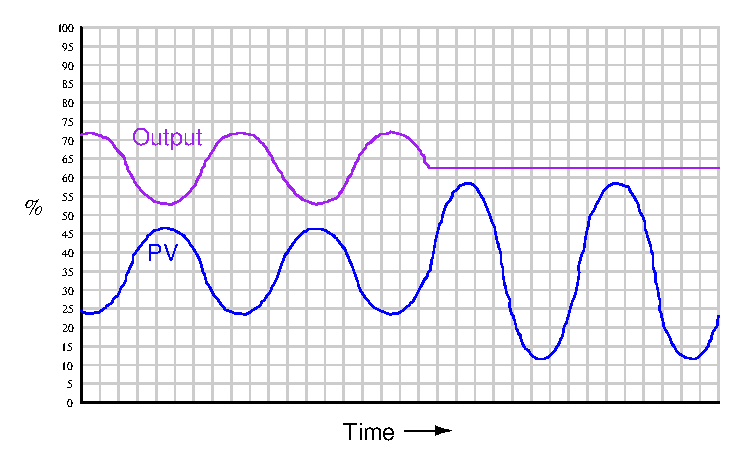
\includegraphics[width=15.5cm]{i01648x01.eps}$$

The result of placing the controller in manual mode surprises you -- if anything, you expected the PV to ``calm down'' rather than become {\it more} cyclic!  Determine what this trend tells us about the nature of the cycling problem and its potential cause(s).  Also, explain why placing the controller in manual mode was a good idea for diagnostic purposes.

\vskip 10pt

If you were the instrument technician who discovered this, what would be your next diagnostic step?

\vskip 20pt \vbox{\hrule \hbox{\strut \vrule{} {\bf Suggestions for Socratic discussion} \vrule} \hrule}

\begin{itemize}
\item{} Generally, the appearance of a nice, {\it sinusoidal} oscillation tells us something specific about the cause of the oscillation.  What does the sinusoidal shape of the oscillation suggest to us?
\item{} Based on this trend graph, can we tell whether this is a direct-acting or a reverse-acting controller?  If so, which action is it?
\item{} Based on this trend graph, can we identify the dominant control action (P, I, or D) of the controller?  If so, identify which action is doing most of the work here.
\item{} Based on this trend graph, can we identify the amount of gain (P action) is programmed in the controller?  If so, estimate the controller's gain value.
\item{} Based on this trend graph, can we identify the amount of gain in the process?  If so, estimate the process gain value.
\end{itemize}

\underbar{file i01648}
%(END_QUESTION)





%(BEGIN_ANSWER)

Whatever the problem is, it is {\it not} in this loop controller! 

%(END_ANSWER)





%(BEGIN_NOTES)

The fact that the cycling worsens when the controller is placed in manual mode tells us that the cycling is coming from something other than the controller, rather than the controller being the cause of the cycling.  What is most likely going on here is some {\it other} control loop in the larger system is cycling, placing a cyclic {\it load} on this controller that this controller cannot neutralize while in automatic mode.  That is what the sinusoidal shape suggests: an over-tuned controller oscillating at its ultimate period (frequency).

It is possible that we could improve the situation by increasing the aggressiveness of this controller, so that it reacts more swiftly and more effectively to the sinusoidal load, but the primary cause of the problem is definitely something else in the process that is oscillating.

%INDEX% Process troubleshooting: diagnosing problem via trend recording

%(END_NOTES)


